\section{From Candidates to Program}

    The way we approach this is to not have any assumptions as to why the compiler chooses to do a particular reordering in the program. 
    We instead only check if the reoredered program can have its observable behaviors as a subset of the original. 
    This ensures that the algorithm for the compiler optimization need not change, but that our set of conditions will just be additional checks that can be done before actually doing the reordering. 
    Such an approach makes reordering parametric to the memory model. 
    
    The downside is that this approach will be conservative as we use no information as to why a particular set of events are reordered. We do not compare and contrast in details the perks of both approaches. This is beyond the scope of this thesis.

    \subsection{Addressing Programs with Conditionals}
        We first consider the elimination of write in programs with conditional branches. The following corollary states when doing such an elimination is safe: 

        \begin{corollary}
            Consider a program $P$ and its candidates $C_1, C_2, ... , C_n$ in which events $e$ and $d$ present such that 
            \begin{align*}
                \event{e}{W} \ \wedge \ \event{d}{W} \ \wedge \ \et{e}{uo} \ \wedge \ \reln{e}{ao}{d} \ \wedge \ \Re(e)\!=\!\Re(d)
            \end{align*} . 
            Consider the set of corresponding candidates $C'_1, C'_2, ... , C'_n$ after eliminating $e$ and its corresponding program $P'$. If
            \begin{align*}
                \forall C_{i \in [1,n]}, \forall k \in C_i \ \text{s.t.} \ \reln{e}{ao}{k} \wedge \reln{k}{ao}{d}, \    
                Reord(e,k)  
            \end{align*}
            and
            \begin{align*}
                \nexists C \in P \ \text{s.t.} \ \event{e}{C} \wedge d \notin C
            \end{align*}
            Then the set of observable behaviors of $P'$ is a subset of that of $P$.
        \end{corollary}

        \begin{proof}
            We first prove that the second condition must hold. We show this by proving that if it does not hold, a new observable behavior     can be introduced. 

            Suppose the second condition does not hold, then we have 
            \begin{align*}
                \exists C \in P \ \text{s.t.} \  \event{e}{C} \wedge d \notin C
            \end{align*}

            By Prop \ref{CondB1} and Prop \ref{CondB1}, we can infer that the above holds if $e$ or $d$ are part of a conditional branch. 
            \begin{itemize}
                \item Case 1: $e$ and $d$ both are part of conditionals 

                    If $e$ and $d$ are part of different branches of the same conditional, then we have $\neg \reln{e}{ao}{d}$. Hence this  case need not be considered.     

                    There are remaining four types of this case that we need to consider: 

                    \begin{enumerate}
                        \item Type 1: 

                            \begin{figure}[H]
                                \centering 
                                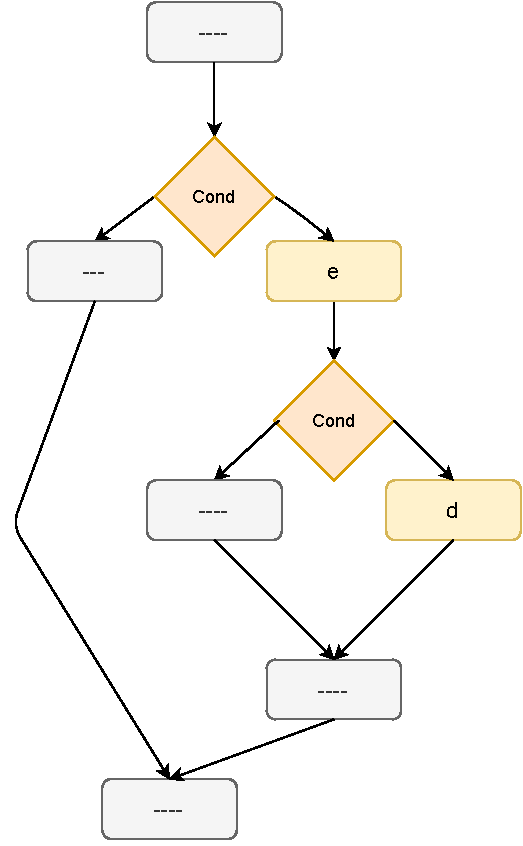
\includegraphics[scale=0.7]{Elimination/ConditionalsProofFig1.pdf}
                                \caption{Type 1:}    
                            \end{figure}
                        
                            From the figure, we can infer by Prop \ref{CondB1} that  
                            \begin{align*}
                                \exists C \in P \ \text{s.t.} \ e \in C \ \wedge \ d \notin C
                            \end{align*}
                            After elimination $e$, we can have a new observable behavior in a candidate not having $d$ from the above property of this case.  

                        \item Type 2: 

                            \begin{figure}[H]
                                \centering 
                                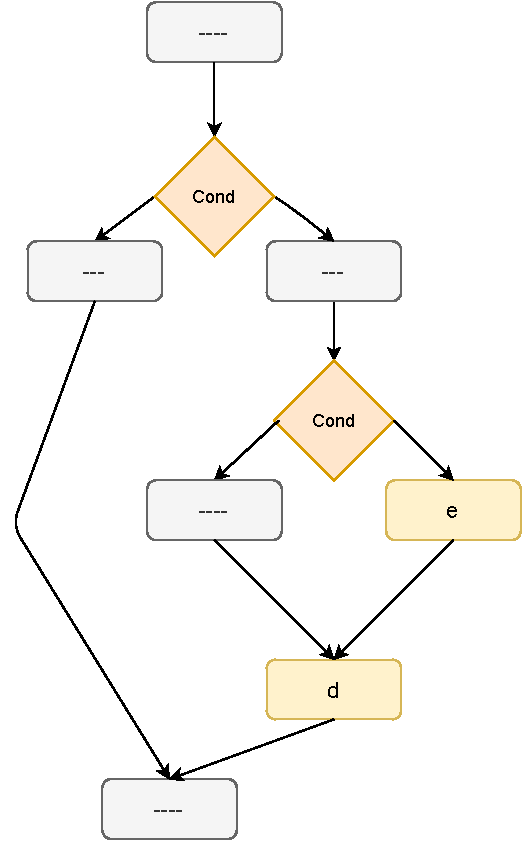
\includegraphics[scale=0.7]{Elimination/ConditionalsProofFig2.pdf}
                                \caption{Type 2:}    
                            \end{figure}
                        
                            From the figure, we can infer by Prop \ref{CondB1} that
                            \begin{align*}
                                \exists C \in P \ \text{s.t.} \ e \notin C \ \wedge \ d \in C
                            \end{align*}
                            After elimination $e$, we cannot have any new observable behavior in a candidate not having $d$ as by Prop \ref {CondB1}, we have for the original program that  
                            \begin{align*}
                                \exists C \in P \ \text{s.t.} \ e \notin C \ \wedge \ d \notin C
                            \end{align*}

                        \item Type 3: 
                        
                            \begin{figure}[H]
                                \centering 
                                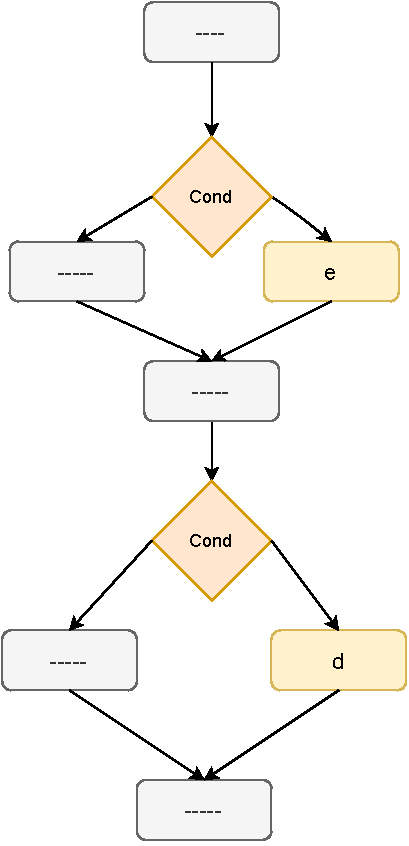
\includegraphics[scale=0.7]{Elimination/ConditionalsProofFig3.pdf}
                                \caption{Type 3:}    
                            \end{figure}

                            If $e$ and $d$ are part of different conditional branches, then by Prop \ref{CondB2} and \ref{CondB1}, we have 
                            \begin{align*}
                                \exists C \in P \ \text{s.t.} \ d \notin C \\ 
                                \exists C \in P \ \text{s.t.} \ e \notin C 
                            \end{align*}
                            After elimination $e$, we can have a new observable behavior in a candidate not having $d$ as above condition states. 
                        
                        \item Type 4: 

                            \begin{figure}[H]
                                \centering 
                                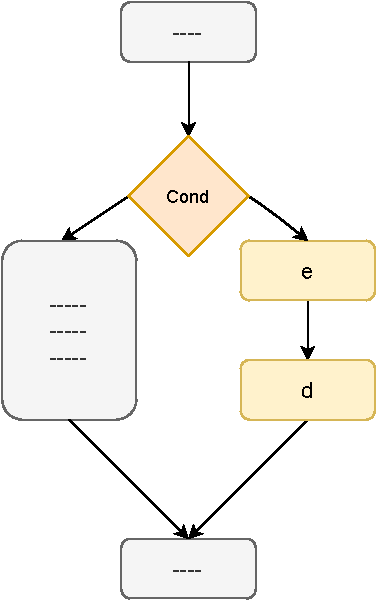
\includegraphics[scale=0.7]{Elimination/ConditionalsProofFig4.pdf}
                                \caption{Type 4:}    
                            \end{figure}

                            From the figure, we can infer by Prop \ref{CondB1} that
                            \begin{align*}
                                \exists C \in P \ \text{s.t.} \ e \notin C \ \wedge \ d \notin C
                            \end{align*}
                            After elimination $e$, we cannot have any new observable behavior in a candidate not having $d$ as we have by Prop \ref{CondB1} that  
                            \begin{align*}
                                e \in C \ \Rightarrow \ d \in C
                            \end{align*}

                            \critic{purple}{Not sure how to come to the above conclusion apart from the fact that its obvious.}

                    \end{enumerate}

                    \critic{red}{Need to refer to part of elimination proof as Coherent Reads would not be triggered anymore for a case and thus we can have a new observable behavior. How to explain this, ask Clark.}

                \item Case 2: $e$ is part of conditional but $d$ is not

                    \begin{figure}[H]
                        \centering 
                        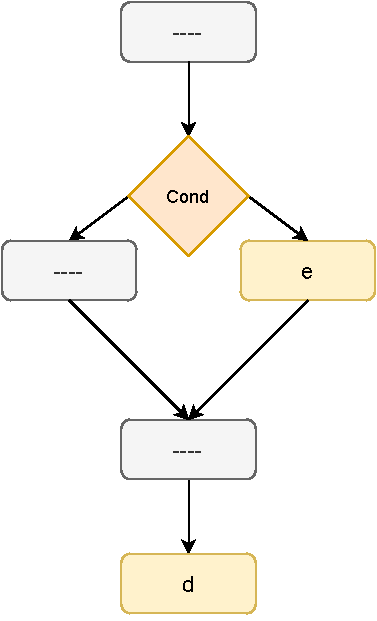
\includegraphics[scale=0.7]{Elimination/ConditionalsProofFig6.pdf}
                        \caption{ }    
                    \end{figure}
                
                
                    By Prop \ref{CondB2} and \ref{CondB1}, we have 
                    \begin{align*}
                        \exists C \in P \ \text{s.t.} \ e \notin C 
                    \end{align*}
                    After elimination $e$, we cannot have a new observable behavior in a candidate due to not having $d$ as above condition states.

                \item Case 3: $d$ is part of a conditional but $e$ is not

                    \begin{figure}[H]
                        \centering 
                        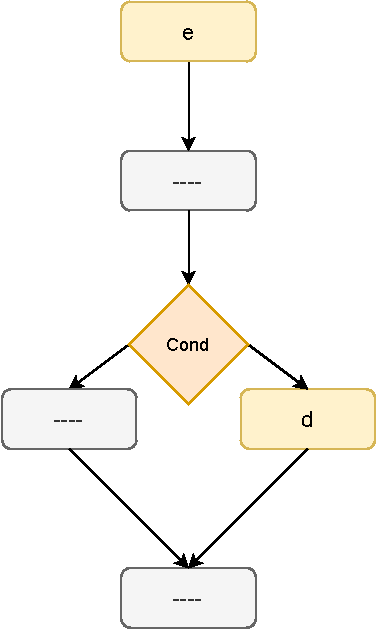
\includegraphics[scale=0.7]{Elimination/ConditionalsProofFig5.pdf}
                        \caption{4:}    
                    \end{figure}

                    By Prop \ref{CondB2} and \ref{CondB1}, we have 
                    \begin{align*}
                        \exists C \in P \ \text{s.t.} \ d \notin C
                    \end{align*}
                    After elimination $e$, we can have a new observable behavior in a candidate not having $d$ as above condition states. 

                    \critic{red}{Need to refer to part of elimination proof as Coherent Reads would not be triggered anymore for a case and thus we can have a new observable behavior. How to explain this, ask Clark.}

                    \critic{purple}{Add the above property to conditionals with two branches also.}

            \end{itemize}

            Now that we have that the second condition must hold, we prove the first condition too must hold. Let $C_i$ and $C_i'$ be the candidates before and after eliminating $e$. From the first condition we have then for $C_i$
            \begin{align*}
                \forall \ k \ \textit{s.t.} \ 
                \reln{e}{ao}{k} \ \wedge \ \reln{k}{ao}{d} \ . \ 
                Reord(e,k).
            \end{align*}
            The above is Corollary 1 (tag properly) for elimination, thus giving us that the observable behaviors of $C_i'$ is a subset of $C_i$. Hence this condition must hold for all candidates from which we eliminate $e$. 

            By property of unions of sets, we can conclude that the set of Observable Behaviors of $P'$ is a subset of that of $P$.

            Hence proved.

            \critic{purple}{We have not given properly the link between Observable Behaviors, Candidate Executions, Candidates and Programs. Perhaps we need to define a function Obs that gives us the set of Observable Behaviors, where the Domain can be a Program, Candidate, or Candidate Execution.}
    \end{proof}

        As far as read elimination goes, since we only need the information of read event that is to be eliminated, we do not need to take cases as above for write elimination. Except there can exist one case, in which the read itself is the conditional check. But what is the resultant code after elimination relies on the intention of the compiler, which can be the following:
        \begin{itemize}
            \item It could be plain dead code elimination, wherein both brnaches of code are eliminated entirely. 
            \item It could also be that the conditonal check always returns the same value, which makes the branch taken to be the same. 
            \item It could also be that the choice of branch does not affect the outcome of the program itself. 
        \end{itemize}
    
        Since we aren't certain of the reason, it is difficult to identify the target code that is inteneded after such an elminiation. Hence we do not address this case. It is also not within the scope of our analysis to conhsder the actual mapping between program and candidates. We would need this to prove that the program does not take a particular conditonal branch in any execution. This is not easy to do without the mapping in our hands. 


    \subsection{Addressing Programs with Loops}
    
        Similar to reordering, for the sake of elimination, we consider programs with just one loop. 
        
        We first consider the simpler case of read elimination within a loop. 
        Eliminating such a read at a program level would imply in every candidate $C^i$ where $i$ denotes the number of iterations, the read $R$ within the loop can be eliminated.
        
        By Thereom 1 of read elimination, we only need the read $R$ to have the type $uo$ to perform such an elimination.
        Thus we can eliminate for each iteration of the loop our intended read. 
        By transitive property of subsets, the resultant candidate will have observable behaviors as a subset of the original. 
        Doing this for all valid canddiates extends to program level.

        Next we consider the case of eliminating writes within a loop. 
        Eliminating such a read at a program level would imply in every candidate $C^i$ where $i$ denotes the number of iterations, the read $W$ within the loop can be eliminated.

        For this, we need to have some write $d$ that can exist in all candidates where $e$ can exist. ($\nexists C \in P \ \text{s.t} \ e \in C \wedge d \notin C$). This condition corresponds to Corollary 2 of elimination, which handles the case of conditonals too. 
        Next, we need to show that in each iteration the write $e$ can be eliminated. We once again have Corollary 2 to show when we can do this. 
        By transitive property of subsets, we can show that the resultant candidate has observable behaviors as a subset of original. 
        Doing this for all valid canddiates extends to program level.
         

        \paragraph{Loop Invariant Code motion}  

            In the previous chapter, we showed that loop invariant code motion cannot be validated by just reordering at the Candidate level. 
            This was because reordering was insufficient to generate the resultant candidate from the original. 
            This however can be done by coupling Reordering with Elimination. 
            
            We first consider the case of reordering a Read outside a loop.
            \begin{corollary}
                \label{LoopInvCodeMotRead1}
                Consider $K$ to be the set of events within a loop in program $P$. Consider $e$ to be a read within the loop. Consider program $P'$ with event $e$ agent ordered before the loop. If
                \begin{gather*}
                    \et{e}{uo} \\
                    \forall k \neq e \in K, \ Reord(k, e) \\ 
                    \nexists C^i \in P \ \text{s.t.} \ e^{j<=i} \notin C                      
                \end{gather*}
                then the set of observable behaviors of $P'$ is a subset of $P$.
            \end{corollary}
            
            \begin{proof}

                We first consider the program with just one iteration. Hence for Candidate $C^1$, we have just $e^1$. 
                We need to ensure that the resultant candidate $C'^1$ such that 
                \begin{align*}
                    \forall k \in K, \ \reln{e}{ao}{k}
                \end{align*}  
                has observable behaviors as a subset of $C^1$

                For every $k \in K$ such that $\reln{k}{ao}{e}$ we have from Condition 2 $Reord(k,e)$. 
                Condition 3, from Prop \ref{CondB1} implies that $e$ is not part of any conditional branch.
                Thus, from Corollary \ref{CorollCodeMotion1} and Corollary \ref{ReordCond}, we can infer that $C'^1$ has observable behaviors as a subset of $C^1$. 
                
                Next, we consider the program with more than one iteration of the loop. 
                We prove this case using induction on the number of reads $e$ that exist due to multiple iterations of the loop. 

                \begin{itemize}

                    \item Base case : number of $e$ = 2
                
                    This case corresponds to candidates of the form $C^2$, thus giving us two reads $e^1$ and $e^2$.
                    From Condition 2, we have
                    \begin{align*}
                        \forall k \in K, \ Reord(k,e^1) \wedge Reord(k, e^2)
                    \end{align*} 
                    From Corollary \ref{CorollCodeMotion1} and Corollary \ref{ReordCond}, we can infer that $C''^2$ has observable behaviors as a subset of $C^2$.
                    To go from $C''^2$ to $C'^2$, note that in $C''^2$ we have $cons(e^1, e^2)$ after reordering them. 
                    From Theorem \ref{ReadElim}, we can eliminate either $e^1$ or $e^2$, thus resulting in $C'^2$ whose observable behaviors is a subset of $C''^2$.
                    
                    By transitive property of subsets we can infer that $C'^2$ has observable behaviors as a subset of $C^2$.
                    
                    \item Inductive case : number of $e$ = n

                    Assume that for all such candidates with $n$ iterations of the loop, the observable behaviors of $C'^n$ is a subset of $C^n$.

                    We now prove using this that it can also hold for number $e$ as $n + 1$. 
                    This case corresponds to candidates of the form $C^{n+1}$, thus giving us $n+1$ reads $e^1, e^2,...,e^{n+1}$.
                    From Condition 2, we have
                    \begin{align*}
                        \forall k \in K, \ Reord(k,e^{n+1})
                    \end{align*}
                    using which we can infer 
                    \begin{align*}
                        \forall k \ \text{s.t.} \ \reln{e^n}{ao}{k} \wedge \reln{k}{ao}{e^{n+1}}, \ Reord(k,e^{n+1})
                    \end{align*}
                    From Corollary \ref{CorollCodeMotion1} and Corollary \ref{ReordCond}, we can infer that $C''^{n+1}$ with $cons(e^n, e^{n+1})$ due to reordering $e^{n+1}$ has observable behaviors as a subset of $C^{n+1}$. 
                    By Theorem \ref{ReadElim}, we can eliminate $e^{n+1}$, thus giving us candidate of the form $C^n$ whose observable behaviors is a subset of $C''^{n+1}$.

                    From our inductive assumption, we can then conclude that $C'^{n+1}$ has observable behaviors as a subset of $C^n$. 
                    By transitive property of subsets, we can infer that $C'^{n+1}$ has observable behaviors as a subset of $C^{n+1}$.

                    \critic{blue}{Mind the notations. Perhaps have another reivew of it to avoid confusion of the reader.}

                    \critic{red}{The argument using Theorem of Read elimination is somewhat cheeky, since we have $cons(e^i, e^{i+1})$ where the two reads are to the same local variable. This additional condition may have to be put in Read Elimination. But let us discuss that with Clark later. }

                \end{itemize}
                
            \end{proof}


            \begin{corollary}
                \label{LoopInvCodeMotRead2}
                Consider $K$ to be the set of events within a loop in program $P$. Consider $e$ to be a read within the loop. Consider program $P'$ with event $e$ agent ordered before the loop. If
                \begin{gather*}
                    \et{e}{uo} \\
                    \forall k \neq e \in K, \ Reord(e, k) \\ 
                    \nexists C^i \in P \ \text{s.t.} \ e^{j<=i} \notin C                      
                \end{gather*}
                then the set of observable behaviors of $P'$ is a subset of $P$.
            \end{corollary}
            
            \begin{proof}

                We first consider the program with just one iteration. Hence for Candidate $C^1$, we have just $e^1$. 
                We need to ensure that the resultant candidate $C'^1$ such that 
                \begin{align*}
                    \forall k \in K, \ \reln{k}{ao}{e}
                \end{align*}  
                has observable behaviors as a subset of $C^1$

                For every $k \in K$ such that $\reln{e}{ao}{k}$ we have from Condition 2 $Reord(e,k)$. 
                Condition 3, from Prop \ref{CondB1} implies that $e$ is not part of any conditional branch.
                Thus, from Corollary \ref{CorollCodeMotion2} and Corollary \ref{ReordCond}, we can infer that $C'^1$ has observable behaviors as a subset of $C^1$. 
                
                Next, we consider the program with more than one iteration of the loop. 
                We prove this case using induction on the number of reads $e$ that exist due to multiple iterations of the loop. 

                \begin{itemize}
                    
                    \item Base case : number of $e$ = 2
                
                    This case corresponds to candidates of the form $C^2$, thus giving us two reads $e^1$ and $e^2$.
                    From Condition 2, we have
                    \begin{align*}
                        \forall k \in K, \ Reord(e^1, k) \wedge Reord(e^2, k)
                    \end{align*} 
                    From Corollary \ref{CorollCodeMotion1} and Corollary \ref{ReordCond}, we can infer that $C''^2$ has observable behaviors as a subset of $C^2$.
                    To go from $C''^2$ to $C'^2$, note that in $C''^2$ we have $cons(e^1, e^2)$ after reordering them. 
                    From Theorem \ref{ReadElim}, we can eliminate either $e^1$ or $e^2$, thus resulting in $C'^2$ whose observable behaviors is a subset of $C''^2$.
                    
                    By transitive property of subsets we can infer that $C'^2$ has observable behaviors as a subset of $C^2$.
                    
                    \item Inductive case : number of $e$ = n

                    Assume that for all such candidates with $n$ iterations of the loop, the observable behaviors of $C'^n$ is a subset of $C^n$.

                    We now prove using this that it can also hold for number $e$ as $n + 1$. 
                    This case corresponds to candidates of the form $C^{n+1}$, thus giving us $n+1$ reads $e^1, e^2,...,e^{n+1}$.
                    From Condition 2, we have
                    \begin{align*}
                        \forall k \in K, \ Reord(e^{n}, k)
                    \end{align*}
                    using which we can infer 
                    \begin{align*}
                        \forall k \ \text{s.t.} \ \reln{e^n}{ao}{k} \wedge \reln{k}{ao}{e^{n+1}}, \ Reord(e^{n}, k)
                    \end{align*}
                    From Corollary \ref{CorollCodeMotion1} and Corollary \ref{ReordCond}, we can infer that $C''^{n+1}$ with $cons(e^n, e^{n+1})$ due to reordering $e^{n+1}$ has observable behaviors as a subset of $C^{n+1}$. 
                    By Theorem \ref{ReadElim}, we can eliminate $e^{n+1}$, thus giving us candidate of the form $C^n$ whose observable behaviors is a subset of $C''^{n+1}$.

                    From our inductive assumption, we can then conclude that $C'^{n+1}$ has observable behaviors as a subset of $C^n$. 
                    By transitive property of subsets, we can infer that $C'^{n+1}$ has observable behaviors as a subset of $C^{n+1}$.

                    \critic{blue}{Mind the notations. Perhaps have another reivew of it to avoid confusion of the reader.}

                    \critic{red}{The argument using Theorem of Read elimination is somewhat cheeky, since we have $cons(e^i, e^{i+1})$ where the two reads are to the same local variable. This additional condition may have to be put in Read Elimination. But let us discuss that with Clark later. }

                \end{itemize}
                
            \end{proof}
            
            Now we consider the case of reordering a write outside a loop:
            \begin{corollary}
                \label{LoopInvCodeMotWrite1}
                Consider $K$ to be the set of events within a loop in program $P$. Consider $e$ to be a read within the loop. Consider program $P'$ with event $e$ agent ordered before the loop. If
                \begin{gather*}
                    \et{e}{uo} \\
                    \forall k \neq e \in K, \ Reord(k, e) \\ 
                    \nexists C^i \in P \ \text{s.t.} \ e^{j<=i} \notin C                      
                \end{gather*}
                then the set of observable behaviors of $P'$ is a subset of $P$.

                \critic{red}{It is interesting to note that we do not need $Reord(e,k)$ which was originally our plan because we needed to eliminate every $e^j$ w.r.t $e^{j+1}$. Because we have $Reord(k,e)$, we can get all the writes to be consecutive to each other. Thus by Theorem 1 directly, we can eliminate them all. We do not require Corollary of Elimination here.}
            \end{corollary}             
            
            \begin{proof}


                We first consider the program with just one iteration. Hence for Candidate $C^1$, we have just $e^1$. 
                We need to ensure that the resultant candidate $C'^1$ such that 
                \begin{align*}
                    \forall k \in K, \ \reln{e}{ao}{k}
                \end{align*}  
                has observable behaviors as a subset of $C^1$

                For every $k \in K$ such that $\reln{k}{ao}{e}$ we have from Condition 2 $Reord(k,e)$. 
                Condition 3, from Prop \ref{CondB1} implies that $e$ is not part of any conditional branch.
                Thus, from Corollary \ref{CorollCodeMotion1} and Corollary \ref{ReordCond}, we can infer that $C'^1$ has observable behaviors as a subset of $C^1$. 
                
                Next, we consider the program with more than one iteration of the loop. 
                We prove this case using induction on the number of reads $e$ that exist due to multiple iterations of the loop. 


                \begin{itemize}

                    \item Base case : number of $e$ = 2
                
                    This case corresponds to candidates of the form $C^2$, thus giving us two reads $e^1$ and $e^2$.
                    From Condition 2, we have
                    \begin{align*}
                        \forall k \in K, \ Reord(k,e^1) \wedge Reord(k, e^2)
                    \end{align*} 
                    From Corollary \ref{CorollCodeMotion1} and Corollary \ref{ReordCond}, we can infer that $C''^2$ has observable behaviors as a subset of $C^2$.
                    To go from $C''^2$ to $C'^2$, note that in $C''^2$ we have $cons(e^1, e^2)$ after reordering them. 
                    From Theorem \ref{WriteElim}, we can eliminate $e^1$, thus resulting in $C'^2$ whose observable behaviors is a subset of $C''^2$.
                    
                    By transitive property of subsets we can infer that $C'^2$ has observable behaviors as a subset of $C^2$.
                    
                    \item Inductive case : number of $e$ = n

                    Assume that for all such candidates with $n$ iterations of the loop, the observable behaviors of $C'^n$ is a subset of $C^n$.

                    We now prove using this that it can also hold for number $e$ as $n + 1$. 
                    This case corresponds to candidates of the form $C^{n+1}$, thus giving us $n+1$ reads $e^1, e^2,...,e^{n+1}$.
                    From Condition 2, we have
                    \begin{align*}
                        \forall k \in K, \ Reord(k,e^{n+1})
                    \end{align*}
                    using which we can infer 
                    \begin{align*}
                        \forall k \ \text{s.t.} \ \reln{e^n}{ao}{k} \wedge \reln{k}{ao}{e^{n+1}}, \ Reord(k,e^{n+1})
                    \end{align*}
                    From Corollary \ref{CorollCodeMotion1} and Corollary \ref{ReordCond}, we can infer that $C''^{n+1}$ with $cons(e^n, e^{n+1})$ due to reordering $e^{n+1}$ has observable behaviors as a subset of $C^{n+1}$. 
                    By Theorem \ref{WriteElim}, we can eliminate $e^{n+1}$, thus giving us candidate of the form $C^n$ whose observable behaviors is a subset of $C''^{n+1}$.

                    From our inductive assumption, we can then conclude that $C'^{n+1}$ has observable behaviors as a subset of $C^n$. 
                    By transitive property of subsets, we can infer that $C'^{n+1}$ has observable behaviors as a subset of $C^{n+1}$.

                    \critic{blue}{Mind the notations. Perhaps have another reivew of it to avoid confusion of the reader.}

                \end{itemize}

            \end{proof}


            \begin{corollary}
                \label{LoopInvCodeMotWrite2}
                Consider $K$ to be the set of events within a loop in program $P$. Consider $e$ to be a read within the loop. Consider program $P'$ with event $e$ agent ordered before the loop. If
                \begin{gather*}
                    \et{e}{uo} \\
                    \forall k \neq e \in K, \ Reord(e, k) \\ 
                    \nexists C^i \in P \ \text{s.t.} \ e^{j<=i} \notin C                      
                \end{gather*}
                then the set of observable behaviors of $P'$ is a subset of $P$.

                \critic{red}{It is interesting to note that we do not need $Reord(e,k)$ which was originally our plan because we needed to eliminate every $e^j$ w.r.t $e^{j+1}$. Because we have $Reord(k,e)$, we can get all the writes to be consecutive to each other. Thus by Theorem 1 directly, we can eliminate them all. We do not require Corollary of Elimination here.}
            \end{corollary}             
            
            \begin{proof}


                We first consider the program with just one iteration. Hence for Candidate $C^1$, we have just $e^1$. 
                We need to ensure that the resultant candidate $C'^1$ such that 
                \begin{align*}
                    \forall k \in K, \ \reln{k}{ao}{e}
                \end{align*}  
                has observable behaviors as a subset of $C^1$

                For every $k \in K$ such that $\reln{k}{ao}{e}$ we have from Condition 2 $Reord(e, k)$. 
                Condition 3, from Prop \ref{CondB1} implies that $e$ is not part of any conditional branch.
                Thus, from Corollary \ref{CorollCodeMotion1} and Corollary \ref{ReordCond}, we can infer that $C'^1$ has observable behaviors as a subset of $C^1$. 
                
                Next, we consider the program with more than one iteration of the loop. 
                We prove this case using induction on the number of reads $e$ that exist due to multiple iterations of the loop. 


                \begin{itemize}

                    \item Base case : number of $e$ = 2
                
                    This case corresponds to candidates of the form $C^2$, thus giving us two reads $e^1$ and $e^2$.
                    From Condition 2, we have
                    \begin{align*}
                        \forall k \in K, \ Reord(e^1, k) \wedge Reord(e^2, k)
                    \end{align*} 
                    We also have from property of loops that $\reln{e^1}{ao}{e^2}$.
                    From Corollary \ref{CorolWriteElim}, we can eliminate $e^1$, giving us $C''^2$ whose observable behaviors as a subset of $C^2$.  
                    From Corollary \ref{CorollCodeMotion2} and Corollary \ref{ReordCond}, we can reorder $e^2$ outside the loop thus giving us $C'^2$ whose observable behaviors as a subset of $C''^2$.
                    
                    By transitive property of subsets we can infer that $C'^2$ has observable behaviors as a subset of $C^2$.
                    
                    \item Inductive case : number of $e$ = n

                    Assume that for all such candidates with $n$ iterations of the loop, the observable behaviors of $C'^n$ is a subset of $C^n$.

                    We now prove using this that it can also hold for number $e$ as $n + 1$. 
                    This case corresponds to candidates of the form $C^{n+1}$, thus giving us $n+1$ reads $e^1, e^2,...,e^{n+1}$.
                    From Condition 2, we have
                    \begin{align*}
                        \forall k \in K, \ Reord(e^{n}, k)
                    \end{align*}
                    using which we can infer 
                    \begin{align*}
                        \forall k \ \text{s.t.} \ \reln{e^n}{ao}{k} \wedge \reln{k}{ao}{e^{n+1}}, \ Reord(e^{n}, k)
                    \end{align*}
                    From Corollart \ref{CorolWriteElim}, we can eliminate $e^{n}$, thus giving us candidate $C^{n}$ whose observable beahviors are a subset of $C^{n+1}$

                    From our inductive assumption, we can then conclude that $C'^{n+1}$ has observable behaviors as a subset of $C^n$. 
                    By transitive property of subsets, we can infer that $C'^{n+1}$ has observable behaviors as a subset of $C^{n+1}$.

                    \critic{blue}{Mind the notations. Perhaps have another reivew of it to avoid confusion of the reader.}

                    \critic{red}{Proof read later.}

                \end{itemize}

            \end{proof}
            
        \paragraph{Reordering two events accross loops} 
            
            Note that we still cannot assert when we can reorder events inside a loop. This would require a proof of redundancy introduction at the candidate level. This is beyond the scope of this thesis. 

            \critic{blue}{Perhaps you can elaborate a bit more on this.}